\section{Theory of the symmetric
circulation}\label{theory-of-the-symmetric-circulation}

The general circulation of the planet has been described in Chapter
\texttt{chp:GeneralCirculation} and we have seen how it is composed of
three distinct zones, the tropics and the two mid-latitudes area. The
dynamics of the zonally symmetric tropical circulation is quite
different from the eddy-dominated, turbulent mid-latitudes so the
question arises what are the limitation to the extent of the symmetric
circulation ? What are the factor that prevent the extension of the
Hadley cell all the way to the poles as it was imagined originally by
Hadley ?

It was recognized early that it is the rotation that modifies the flow
and prevents the direct circulation to each the poles, but a
quantitative investigation of this effect was not done until 1980. In
that year held and Hou published a paper HeldHou1980 that was a decisive
step in the quantification of the symmetric circulation. They considered
the Boussinesq, dry on a hemisphere, with a rigid lid at height H above
the surface. The forcing is chosen to be a relaxation to some sort of
"radiative equilibrium " temperature. Linear vertical diffusion of heat
and momentum is present and a constant diffusivity. Zero stress boundary
condition is imposed at the top, whereas at the ground is proportional
to the surface wind.

The steady equations are:

\[\begin{aligned}
0 = -\nabla\cdot(\bar{v}u) + fv +\frac{u v \tan\theta}{a} + \frac{\partial }{\partial z}\left(\nu\frac{\partial u}{\partial z}\right) \\
0 = -\nabla\cdot(\bar{v}v) - fu -\frac{u^2 \tan\theta}{a} + \frac{\partial }{\partial z}\left(\nu\frac{\partial v}{\partial z}\right) -\frac{1}{a}\frac{\partial \Phi}{\partial \theta}\\
0 = -\nabla\cdot(\bar{v}\Theta) -\frac{1}{\tau}\left(\Theta -\Theta_E\right) + \frac{\partial }{\partial z}\left(\nu\frac{\partial \Theta}{\partial z}\right) \\
0 = -\-\nabla\cdot(\bar{v})\\
\frac{\partial \Phi}{\partial z} = g\frac{\Theta}{\Theta_0}
\end{aligned}\]

where \(\bar{v}= (v,w)\) is the velocity vector in the meridional plane
and

\[\nabla =\left[ \frac{1}{a \cos\theta}\frac{\partial \cos\theta}{\partial \theta}, \frac{\partial }{\partial z}\right]\]

is the gradient operator.

The system will be solved with the boundary conditions

\[\begin{aligned}
&w =0 \quad \frac{\partial u}{\partial z}=\frac{\partial v}{\partial z}=\frac{\partial \Theta}{\partial z}=0 \qquad at \quad z=H \\
&w=0 \quad \frac{\partial \Theta}{\partial z} = 0 , \quad \nu\frac{\partial u}{\partial z} = C u,  \nu\frac{\partial v}{\partial z} = C v \quad \qquad at \quad z=0
\end{aligned}\]

The radiative forcing is chosen to be

\[\frac{\Theta_E(\theta,z)}{\Theta_0} = 1 -\frac{2}{3}\Delta_H P_2(\sin\theta) + \Delta_v\left( \frac{z}{H} - \frac{1}{2}\right)\]

where \(\Theta_0\) is a global mean, \(\Delta_H, \Delta_v\) are
nondimensional constants that represents the fractional change in
temperature from equator to pole and from the top to the bottom,
respectively. \(P_2 = \frac{1}{2}(3x^2-1)\) is the second Legendre
polynomial.

\subsection{The balanced flow}\label{the-balanced-flow}

The equation of motion have a simple solution for the case in which
there is no meridional flow (\(v=0\)). In this case also the vertical
velocity is zero (\(w=0\)) and the temperature is in radiative
equilibrium (\(\Theta = \Theta_E\)), the zonal wind satisfies

{\[\frac{\partial }{\partial z}\left(f u_E + \frac{u_E^2 \tan\theta}{a}\right) = -\frac{g}{a\Theta_0}\frac{\partial \Theta_E}{\partial \theta}\]}

The vertical integration of the momentum equation and using the boundary
condition implies that the zonal wind must be zero at the ground, so we
can integrate eq. \texttt{eq:ue} to obtain

{\[f u_E + \frac{u_E^2 \tan\theta}{a} = -\frac{g}{a\Theta_0}\frac{\partial \Theta_E}{\partial \theta} z = \frac{2\Delta_H}{a} g z \sin\theta \cos\theta\]}

whose solution obeying \(u=0\) at \(z=0\) is then

\[\frac{u_E}{\Omega a} = \left[\left( 1 + \frac{2 R z}{H}\right)^{1/2} - 1 \right]\cos\theta \qquad R = \frac{gH\Delta_H}{\Omega^2 a^2}\]

This distribution is in radiative equilibrium. Note that this is
solution has a westerly wind everywhere at the surface, including the
equator.

\subsection{Hide's theorem}

However this solution has some difficulty. Considering again the zonal
momentum equation

\[-\nabla\cdot(\vec{v} M) + \frac{\partial }{\partial z}\left(\nu\frac{\partial M}{\partial z}\right) = 0\]

where

\[M = \Omega a^2 \cos^2\theta + u a \cos\theta\]

is the angular momentum. We can ask ourselves where it can have a
maximum. Hide showed that his maximum cannot be in the interior of the
fluid. Assume infact that such a maximum exist, then integration around
a closed circuit sufficiently close to the maximum will get

\[\int\nabla\cdot(\vec{v}\, M) dl \approx M \int\nabla\cdot(\vec{v}) =0\]

for incompressibility, whereas the integral of the diffusion will not be
zero. In practice, a maximum in the interior will be diffused away and
the advection will not be capable to counteract. Instead it is possible
to have a maximum close to the surface by vertically integrating the
momentum equation where it is compensated by the stress boundary
condition. The same condition will require that \(u \leqslant 0\) at the
surface. It follows that the angular momentum \(M\) must be always
smaller than its equatorial maximum (\(\Omega a^2\)) everywhere,
yielding the condition

\[u \leqslant u_M = \frac{\Omega a \,\mathrm{sin}^{2} \theta}{\,\mathrm{cos}^{} \theta}\]

this is the solution that corresponds to the conservation of angular
momentum.

This means that the radiative solution \(u_E\) cannot be valid in the
region \(u_E > u_M\) or for
\(\theta < \tan^{-1} [(1+2R)^{1/2} -1]^{1/2}]\). In this region a
meridional circulation is required by the conservation of angular
momentum and the \(u_E\) solution that implies meridional velocity zero
(\(v=0\)), cannot be valid. Using \(\Delta_H = 1/3, H = 15km\) we find
\(R \approx 0.2\) and therefore \(\theta \lesssim 27^\circ\). In this
region the meridional velocity \(v\) cannot be zero as required by the
radiative balance.

Because a meridional flow must exist within a certain region close to
the equator, we can be more precise and assume that such circulation
exists up to a certain latitude \(\theta_h\). The poleward high altitude
branch of the circulation conserves angular momentum so
\(u(\theta, H) \approx u_M(\theta)\), but surface drag at the surface is
sufficiently strong that \(u(\theta,0) \approx 0\). Poleward of the
limiting latitude \(\theta_h\) the circulation is zero and in radiative
equilibrium, \(\Theta = \Theta_E, u=u_E\). In a steady state, then

\[f u + \frac{u^2 \tan\theta}{a} = -\frac{1}{a}\frac{\partial \Phi}{\partial \theta}\]

the difference then between the top (\(z=H\)) and the bottom (\(z=0\))
then is given by

\[f[u(H)-u(0)] + \frac{\tan\theta}{a}[u^2(H) - u^2(0)] = -\frac{gH}{a\Theta_0}\frac{\partial \{ \Theta\} }{\partial \theta}\]

where \{ .\} denotes the vertical mean. Inserting the values

\[2\Omega \,\mathrm{sin}^{} \theta \frac{\Omega a}{\,\mathrm{cos}^{} \theta} \,\mathrm{sin}^{2} \theta + \frac{\tan\theta}{a}\frac{\Omega^2 a^2}{\,\mathrm{cos}^{2} \theta} \,\mathrm{sin}^{4} \theta = -\frac{gH}{a\Theta_0}\frac{\partial \{ \Theta\} }{\partial \theta}\]

and integrating from 0 to \(\theta\)

\[\frac{\{ \Theta(0)\} -  \{ \Theta(H)\} }{\Theta_0}\approx \frac{\Omega^2a^2}{2gH}\frac{\,\mathrm{sin}^{4} \theta}{\,\mathrm{cos}^{2} \theta}\]

We will require the continuity of potential temperature at the latitude
\(\theta_h\)

\[\{ \Theta(\theta_h)\} = \{ \Theta_E(\theta_h)\}\]

whereas the conservation of potential temperature requires

\[\int_0^{\theta_h} \{ \Theta\} \,\mathrm{cos}^{} \theta d\theta = \int_0^{\theta_h} \{ \Theta_E\} \,\mathrm{cos}^{} \theta d\theta\]

These two conditions are two equation for \(\{ \Theta(0)\}\) and
\(\theta_h\), assuming small angles

\[\begin{aligned}
\frac{\{ \Theta\} }{\Theta_0} &= \frac{\{ \Theta(0)\} }{\Theta_0}   -\frac{1}{2}\frac{\Omega^2a^2}{gH}\theta^4\\
\frac{\{ \Theta_E\} }{\Theta_0} &= \frac{\{ \Theta_E(0)\} }{\Theta_0} -\Delta_H \theta^2
\end{aligned}\]

and the solution are

\[
\begin{aligned}
&\frac{\{ \Theta(0)\} }{\Theta_0} = \frac{\{ \Theta_E(0)\} }{\Theta_0} -\frac{5}{18} R \Delta_H\\
&\theta_h = \sqrt{\frac{5}{3} R} =\sqrt{\frac{5}{3} \frac{gH\Delta_H}{\Omega^2 a^2}}
\end{aligned}
\]

Inserting the numerical values we get \(\theta_h \approx 26^\circ\).
This value can be compared with Fig. \texttt{fig:802} where it can be
seen that is a pretty good estimate of the poleward edge of the Hadley
cell.

This theory that is based on the conservation of angular momentum and of
energy (via the conservation of potential temperature) then conclude
that the extent of the Hadley cell is proportional to the square root of
the equator-pole temperature gradient and to the square root of the
height of the troposphere. It is instead inversely proportional to the
rotation rate and the radius of the Earth, larger planets or faster
planets will get smaller hadley cells, whereas slower planets will
result in larger Hadley cells.

\begin{figure}
\centering
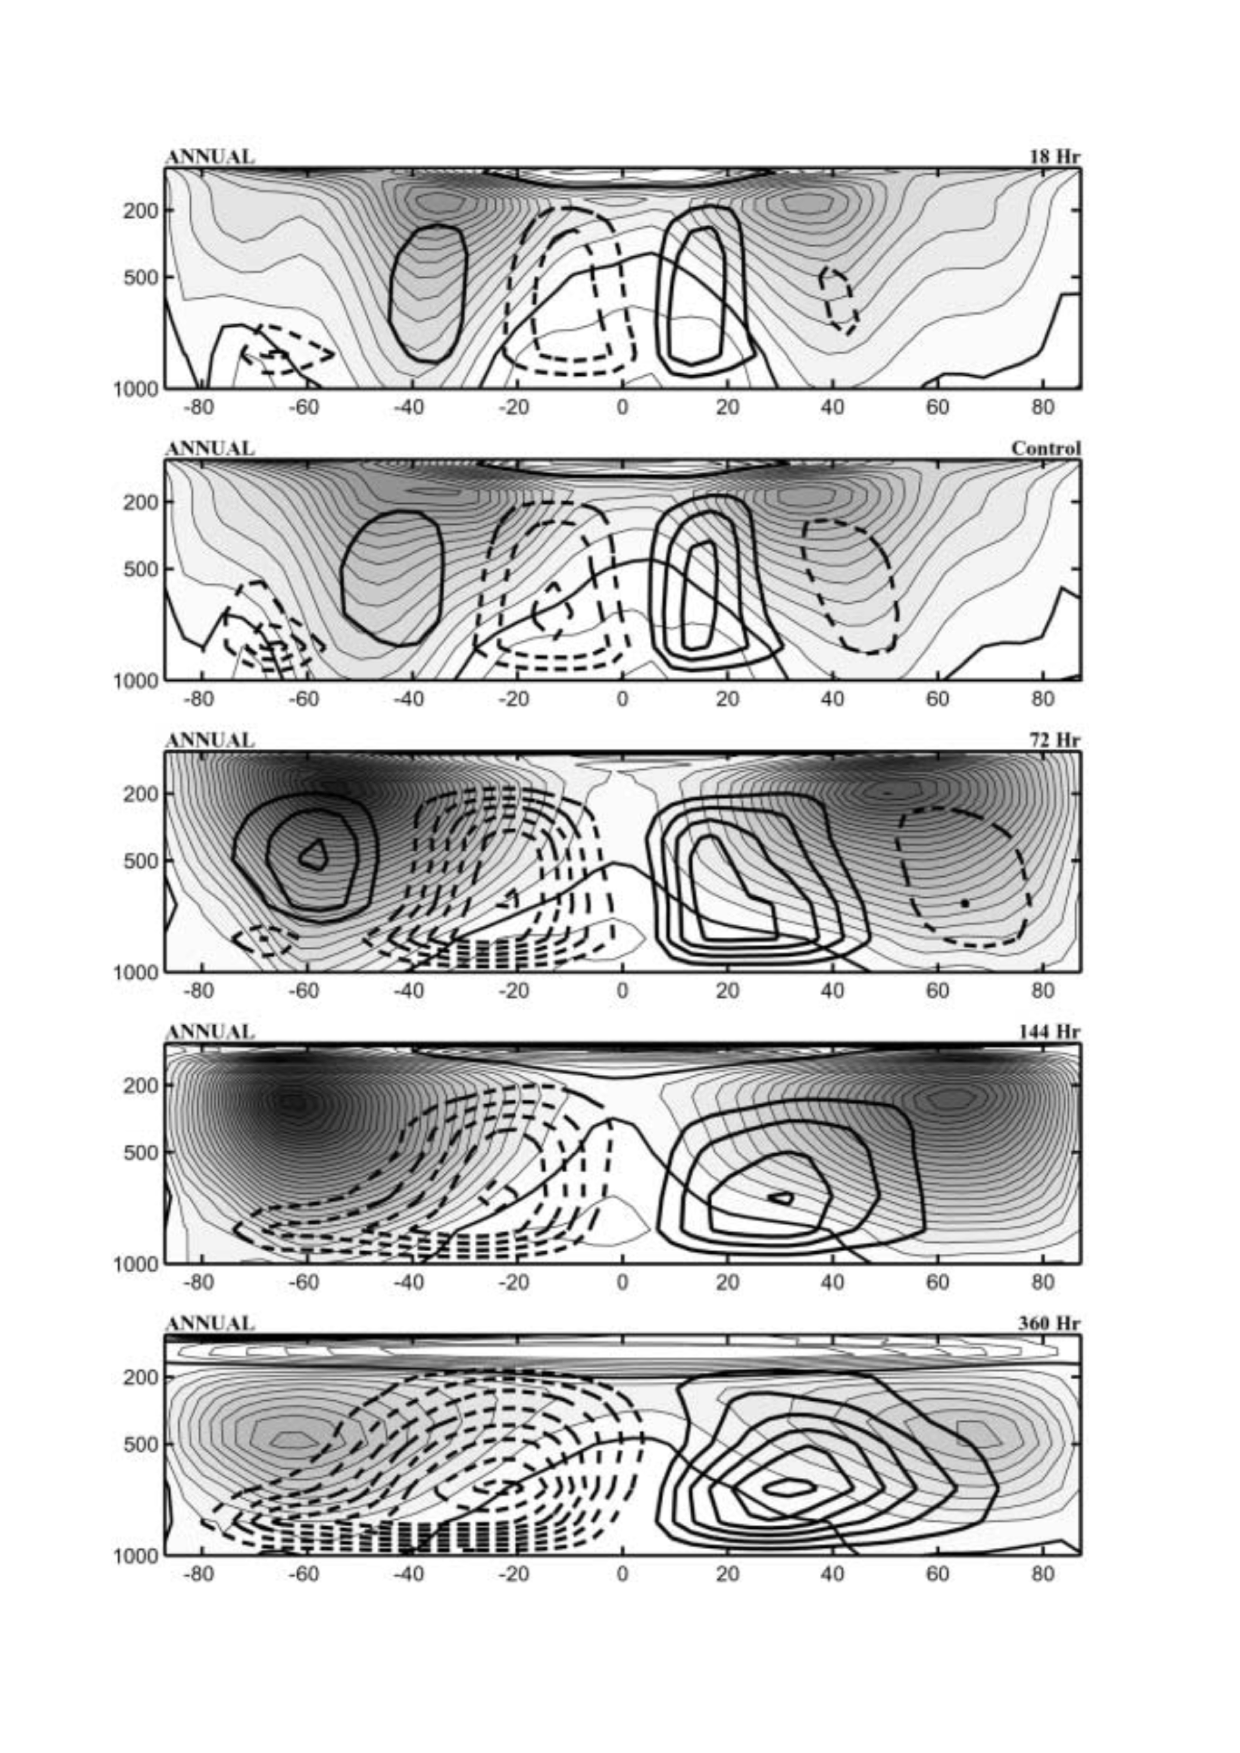
\includegraphics[width = .7 \textwidth]{figs/GD/Rot1.png}
\caption{}
\label{fig:}
\end{figure}

Numerical models can be used to investigate these hypothesis. Fig.
Navarra2002 shows the result of such an experiment performed using a
state of the art general circulation model. The panels show the
meridional streamfunction and the zonal wind for a set of experiments
where the rotation rate of the Earth has been slowed down. It is
possible to see how the Hadley cell grows in extent as the planet slows
and the maximu of the zonal wind shift accordingly poleward. For the
conservation of angular momentum as the jet is squeezed towards the
poles it accelerates, until for very slow rotations, the Hadley cell is
so efficient in transporting momentum that it becomes weaker.

The numerical model gives also the opportunity to investigate the
processes through which the direct circulation breaks down and a
different circulation regime sets up. It is clear i fact that the
theoretical model is highly simplified, especially in the neglect of
transients and theirs variations. From all our discussion on the
importance of transients it is to be expected that they would indeed
play a crucial role also in determining the dynamics of the symmetric
circulation. Fig. \texttt{fig:803} show the numerical equivalent of a
famous laboratory experiment in which a rotating tank is slowly
accelerated while at same time a temperature gradient from the axis of
rotation of the tank toward the external circumference is maintained.
Baroclinic instabilities develop and wavy patterns becomes visible.

In the case of the numerical model all important information is
available and for instance we can see here the meridional transport of
momentum as a function of time , broken in the mean meridional
transport, the transient eddy transport and the stationary wave
transport. The time scale is arbitrary and the model is undergoing a
series of acceleration steps in the rotation rate from 240 hours to 144
hours and then to 72. What we can see is at at the very slow rate the
mean meridional circulation is doing most of the work and there are
almost no transient present. Nothing happens at the 240-144 transition,
but at the next change, from 144 to 72 hours rotation, the eddies start
to appear vigorously and the mean meridional circulation shrinks toward
the equator. This is a demonstration of the unstable nature of the
meridional circulation with respect the rotation rate.

\begin{figure}
\centering
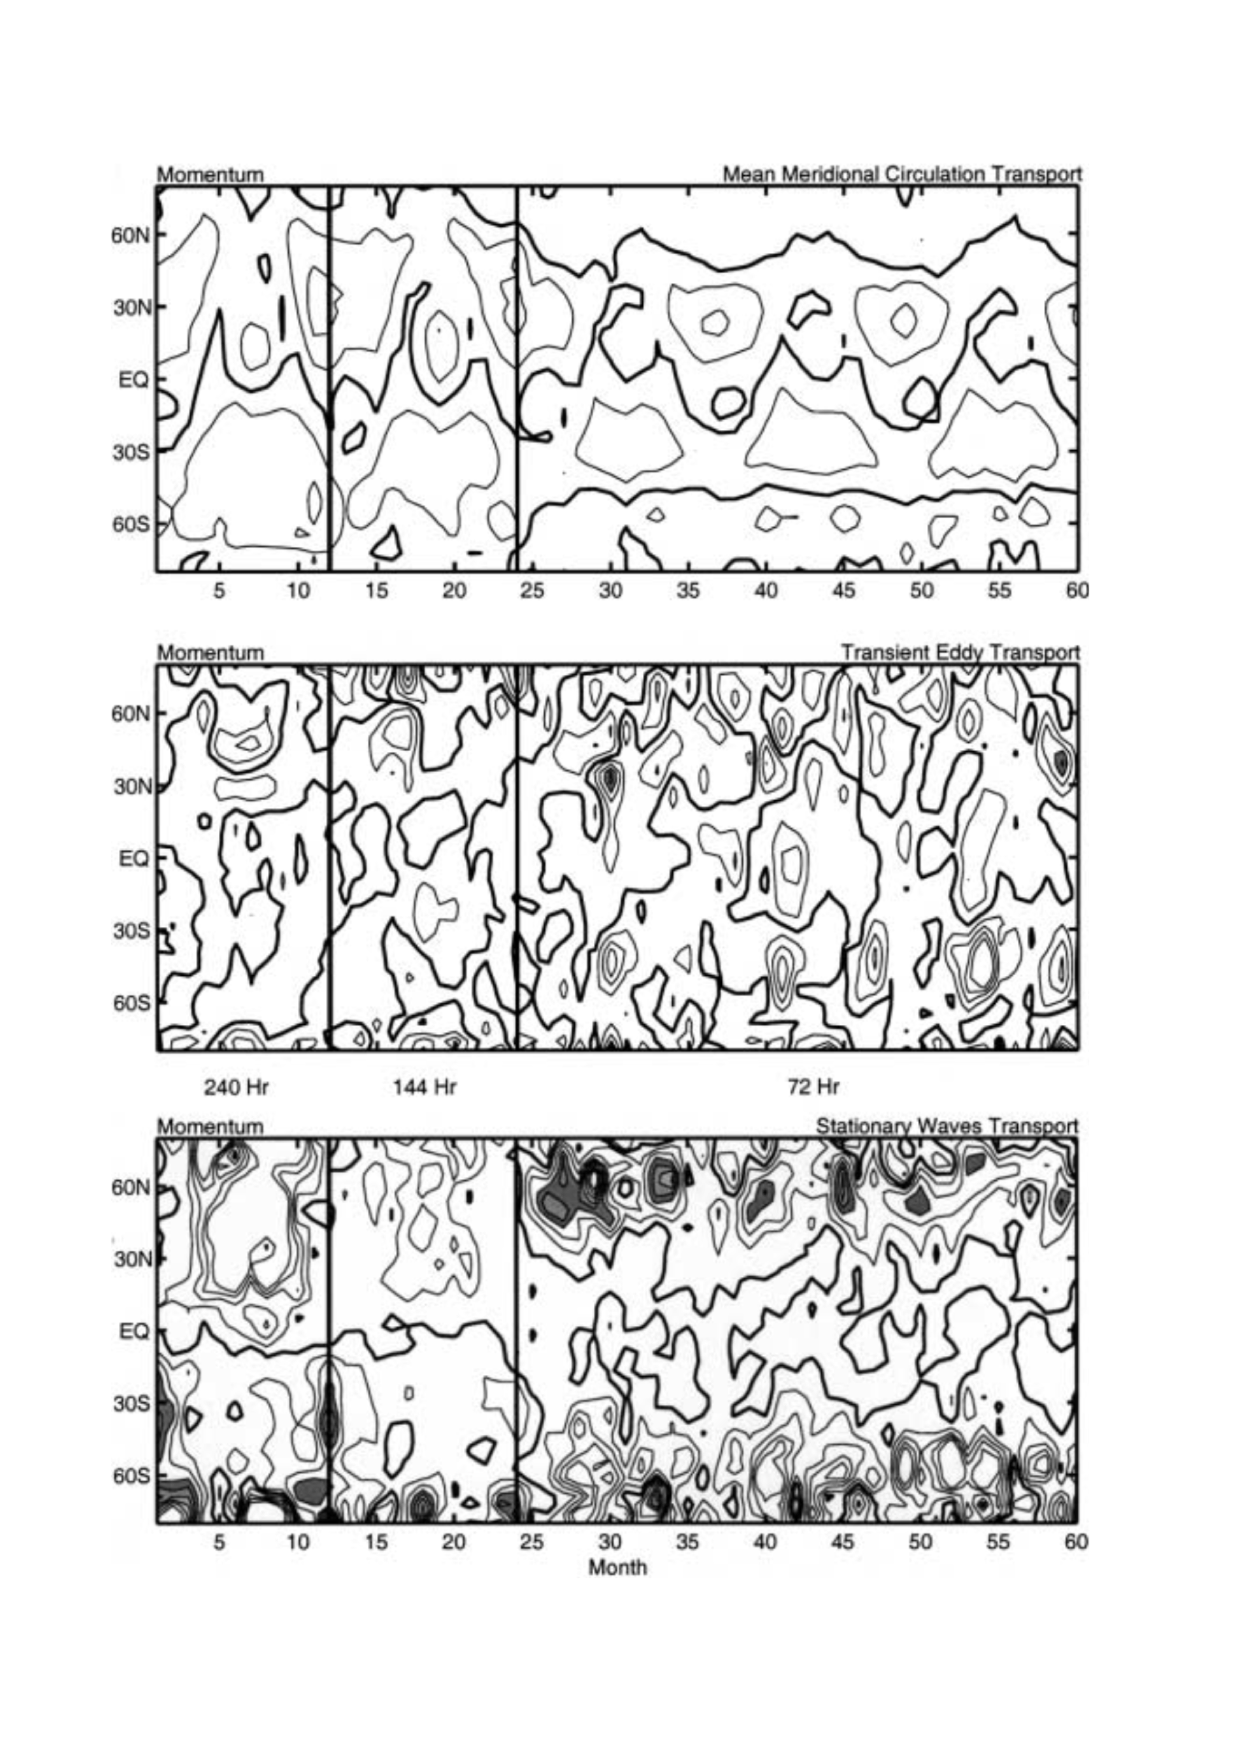
\includegraphics[width = .7 \textwidth]{figs/GD/Rot2.png}
\caption{Stability of the Hadley Cell}
\label{fig:}
\end{figure}


